%%%%%%%%%%%%%%%%%%%%%%%%%%%%%%%%%%%%%%%%%%%%%%%%%%%%%%%%%%%%%%%%%%%
%%% Documento LaTeX 																						%%%
%%%%%%%%%%%%%%%%%%%%%%%%%%%%%%%%%%%%%%%%%%%%%%%%%%%%%%%%%%%%%%%%%%%
% Título:		Capítulo 3
% Autor:  	Ignacio Moreno Doblas
% Fecha:  	2014-02-01, actualizado 2019-11-11
% Versión:	0.5.0
%%%%%%%%%%%%%%%%%%%%%%%%%%%%%%%%%%%%%%%%%%%%%%%%%%%%%%%%%%%%%%%%%%%
% !TEX root = A0.MiTFG.tex

\section{Segunda iteración: Funcionalidad básica}
    \subsection{Resumen}
        La segunda iteración gira en torno a la creación de un primer prototipo funcional que realice, aunque de forma parcial y poco intuitiva, las funciones deseadas para el producto final.

        Centrarse únicamente en la funcionalidad a esta altura del proyecto favorece a reducir el tiempo invertido en pulir detalles que no son realmente necesarios en esta fase tan temprana, economizando el tiempo de desarrollo.

    \subsection{Requisitos}
        Los requisitos a realizar en esta iteración son el 1.3.1, el 1.3.2 y el 2.3 de la tabla de requisitos iniciales (Tabla \ref{tab:Requisitos}). Además, derivado de la iteración anterior, se va a implementar el requisito 1.5 de la tabla completa. (TODO: Cita tabla final). Estos requisitos dan lugar a las siguientes tareas:
    
        \begin{enumerate}
            \item Implementar un mecanismo por el que seleccionar el fichero de entrada.
            \item Implementar la interfaz para los algoritmos de detección.
            \begin{enumerate}
                \item Almacenar la señal de entrada en un buffer.
                \item Definir la interfaz
            \end{enumerate}
            \item Mostrar los resultados del análisis en el panel de usuario.
        \end{enumerate}
        
    \subsection{Desarrollo}
        
        La primera tarea se ha resuelto mediante el empleo de un "QListView"  (TODO:  referencia https://doc.qt.io/archives/qt-4.8/qlistview.html) al que se le ha configurado una carpeta raíz donde se colocarán todos los ficheros de datos junto con unos filtros para que solo muestre estos. Haciendo uso del SLOT \char`_clicked se puede obtener la ruta al fichero que clickea el usuario dentro del widget, permitiendo pasarla como parámetro a la función de lectura implementada en la anterior iteración. 
        
        \begin{figure}[H] 
                \centering
                        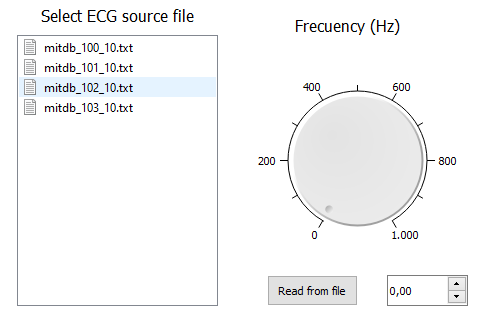
\includegraphics[width = 0.8 \linewidth]{figuras/fileView.png}
                \caption{Estado de la configuración en el panel de control tras la finalización de la segunda iteración.}
                \label{fig:fileView}
        \end{figure}
        
        Para la tarea 2.a se ha implementado un buffer circular empleando una estructura que contiene un array de tipo int32 de 1024 posiciones y una variable para indicar el índice 0 relativo llamada “Head”, una vez inicializado este índice apunta al espacio de memoria donde está almacenado el dato más reciente. Además se proveen dos funciones auxiliares encargadas de introducir y leer elementos del buffer respecto a la posición de la variable Head. 
        
        La función encargada de introducir nuevas muestras modifica el Head del buffer para mantener el estado actualizado, su funcionamiento se explica en el diagrama \ref{fig:bufferDiagramAppend}. 
    
        \begin{figure}[H] 
                \centering
                        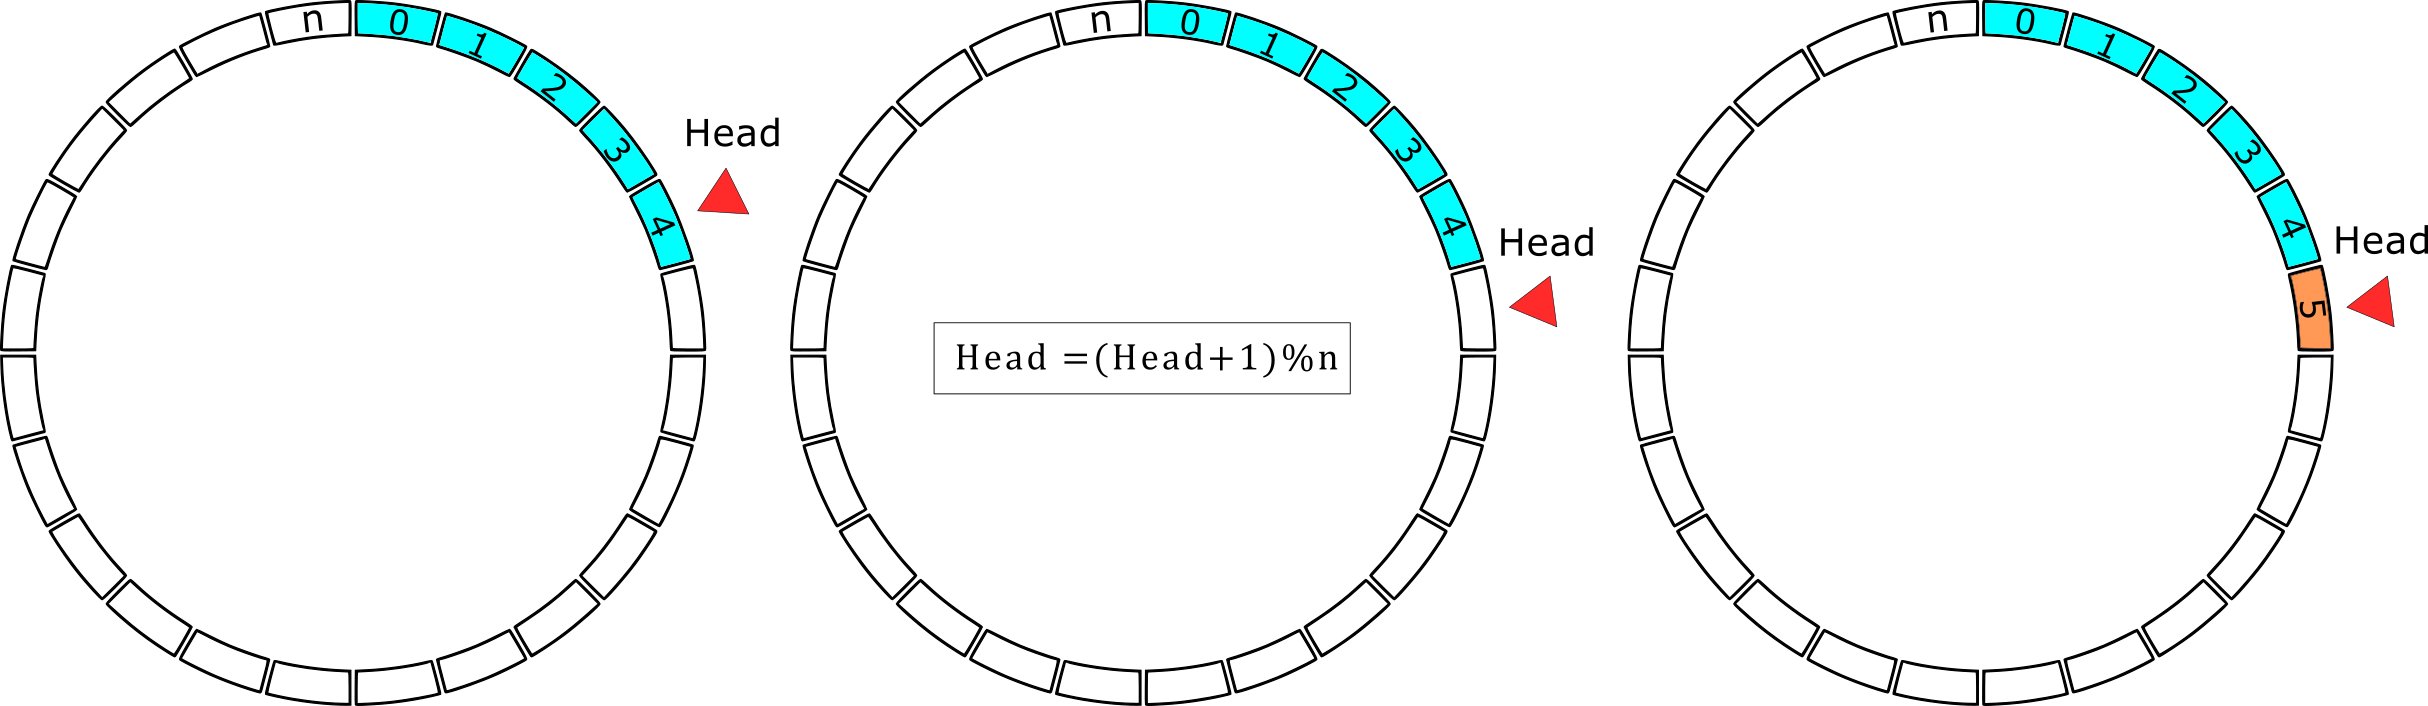
\includegraphics[width = \linewidth]{figuras/bufferAppend.png}
                \caption{Funcionamiento de \char`"AppendSample", función encargada de introducir muestras en el buffer.}
                \label{fig:bufferDiagramAppend}
        \end{figure}
        
        La función encargada de extraer las muestras simplemente recorre el array de forma relativa a la posición del Head como si se tratara de un array normal, retirando del usuario la necesidad de controlar los límites de este. Su funcionamiento está explicado en el diagrama \ref{fig:bufferDiagramGet}.
        
        \begin{figure}[H]
                \centering
                        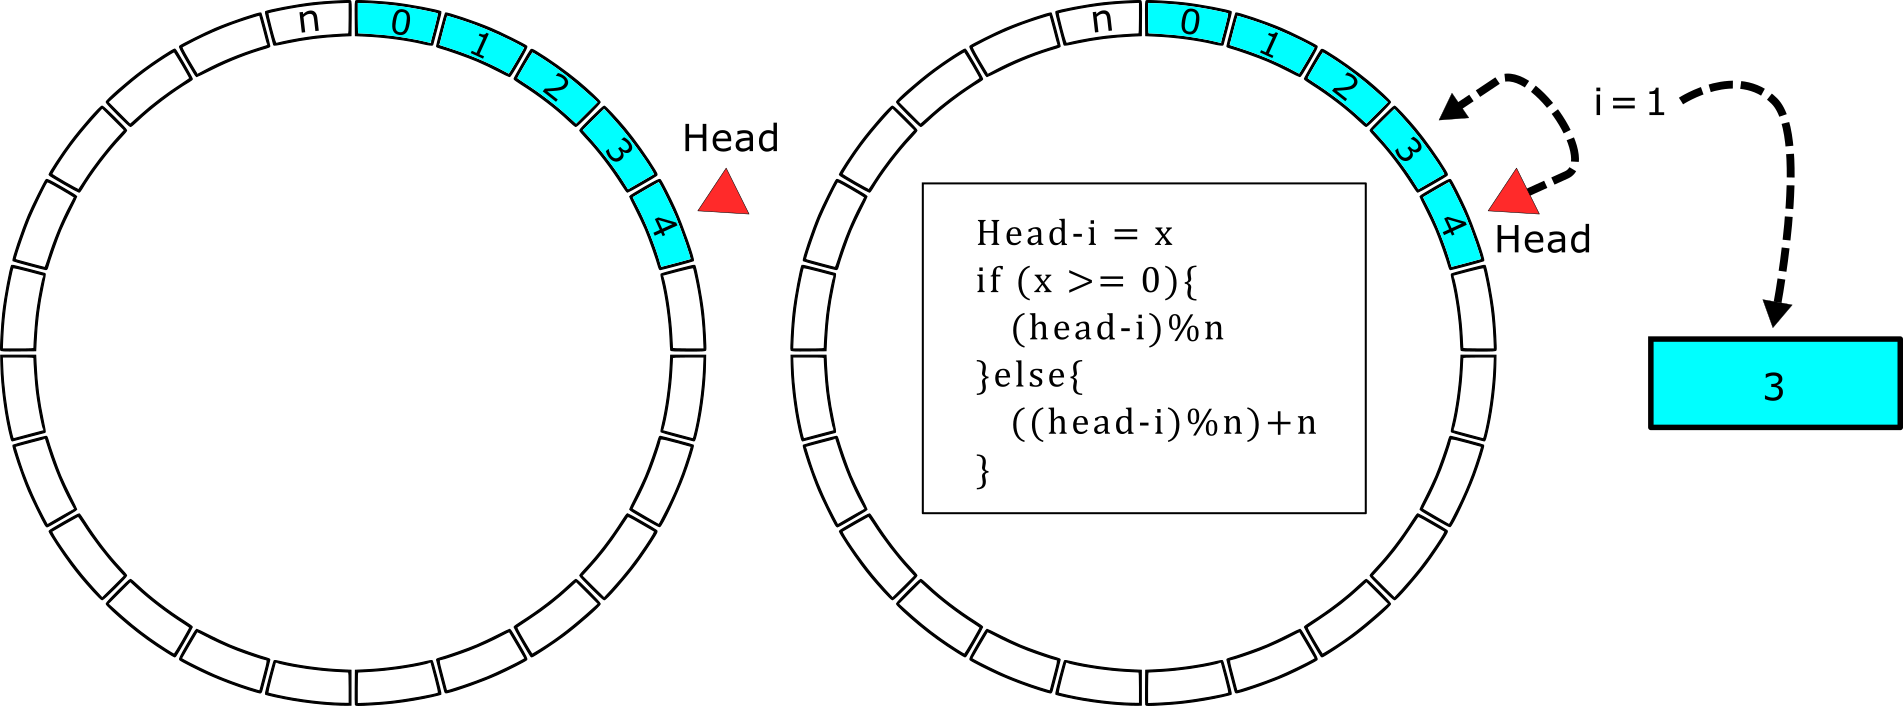
\includegraphics[width = 0.9 \linewidth]{figuras/bufferGet.png}
                \caption{Funcionamiento de "GetSample", función en cargada de extraer las muestras del buffer.}
                \label{fig:bufferDiagramGet}
        \end{figure}
        
        Respecto a la tarea 2.b, si bien no es posible generar una Interfaz propiamente dicha por ser un concepto procedente de la programación orientada a objetos, lo que se trata de lograr es limitar todas las modificaciones que deberá hacer un futuro usuario para introducir su algoritmo a un solo fichero, evitando la necesidad de modificar las llamadas a las funciones en otros ficheros de código. 

        La implementación se ha realizado mediante punteros a funciones. Se ha definido un tipo correspondiente a un puntero a una función con la firma establecida. De esta forma el usuario puede asignar al puntero cualquier función que desarrolle mientras satisfaga la firma impuesta por el mismo, haciendo las veces de interfaz.
        
        En el extracto \ref{code:interface} puede observarse de forma compacta la implementación del funcionamiento previamente descrito. 
        
        \code{Abstracto de la interfaz para el algoritmo del usuario.}{code/interface.cpp}{code:interface}{C++}

        Para la tercera tarea se han decidido implementar varios mecanismos para mostrar los resultados al usuario. Se ha añadido una gráfica empleando el widget QwtPlot donde se muestra la señal ECG leída del fichero en tiempo real. Sobre ella se dibujan los picos R detectados por el algoritmo. Además se ofrece la posibilidad de dibujar el threshold de detección si el algoritmo emplea uno y un recuadro donde se muestra el valor de la tasa cardíaca instantánea medida. En la figura \ref{fig:resultsBasic} puede observarse el formato de salida.

        \begin{figure}[H]
                \centering
                        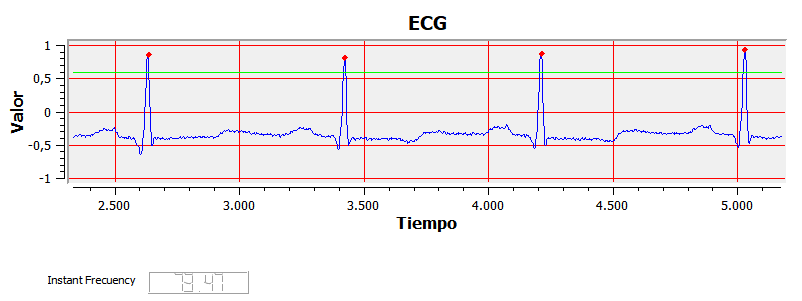
\includegraphics[width =\linewidth]{figuras/ResultsBasic.png}
                \caption{Gráfica que muestra los resultados del análisis llevado a cabo por el algoritmo.}
                \label{fig:resultsBasic}
        \end{figure}
        
    \subsection{Pruebas}
        
        La prueba de la tarea 1 de esta iteración se ha realizado simplemente proveyendo al programa con dos ficheros diferente y mediante el selector leer sus frecuencias. Puesto que la lectura de la frecuencia desde un fichero estaba testeada desde la iteración anterior, esto es suficiente para probar el funcionamiento del selector de ficheros.La figura \ref{fig:fileSelectorTest} se adjunta como prueba del test.

        \begin{figure}[H]
                \centering
                        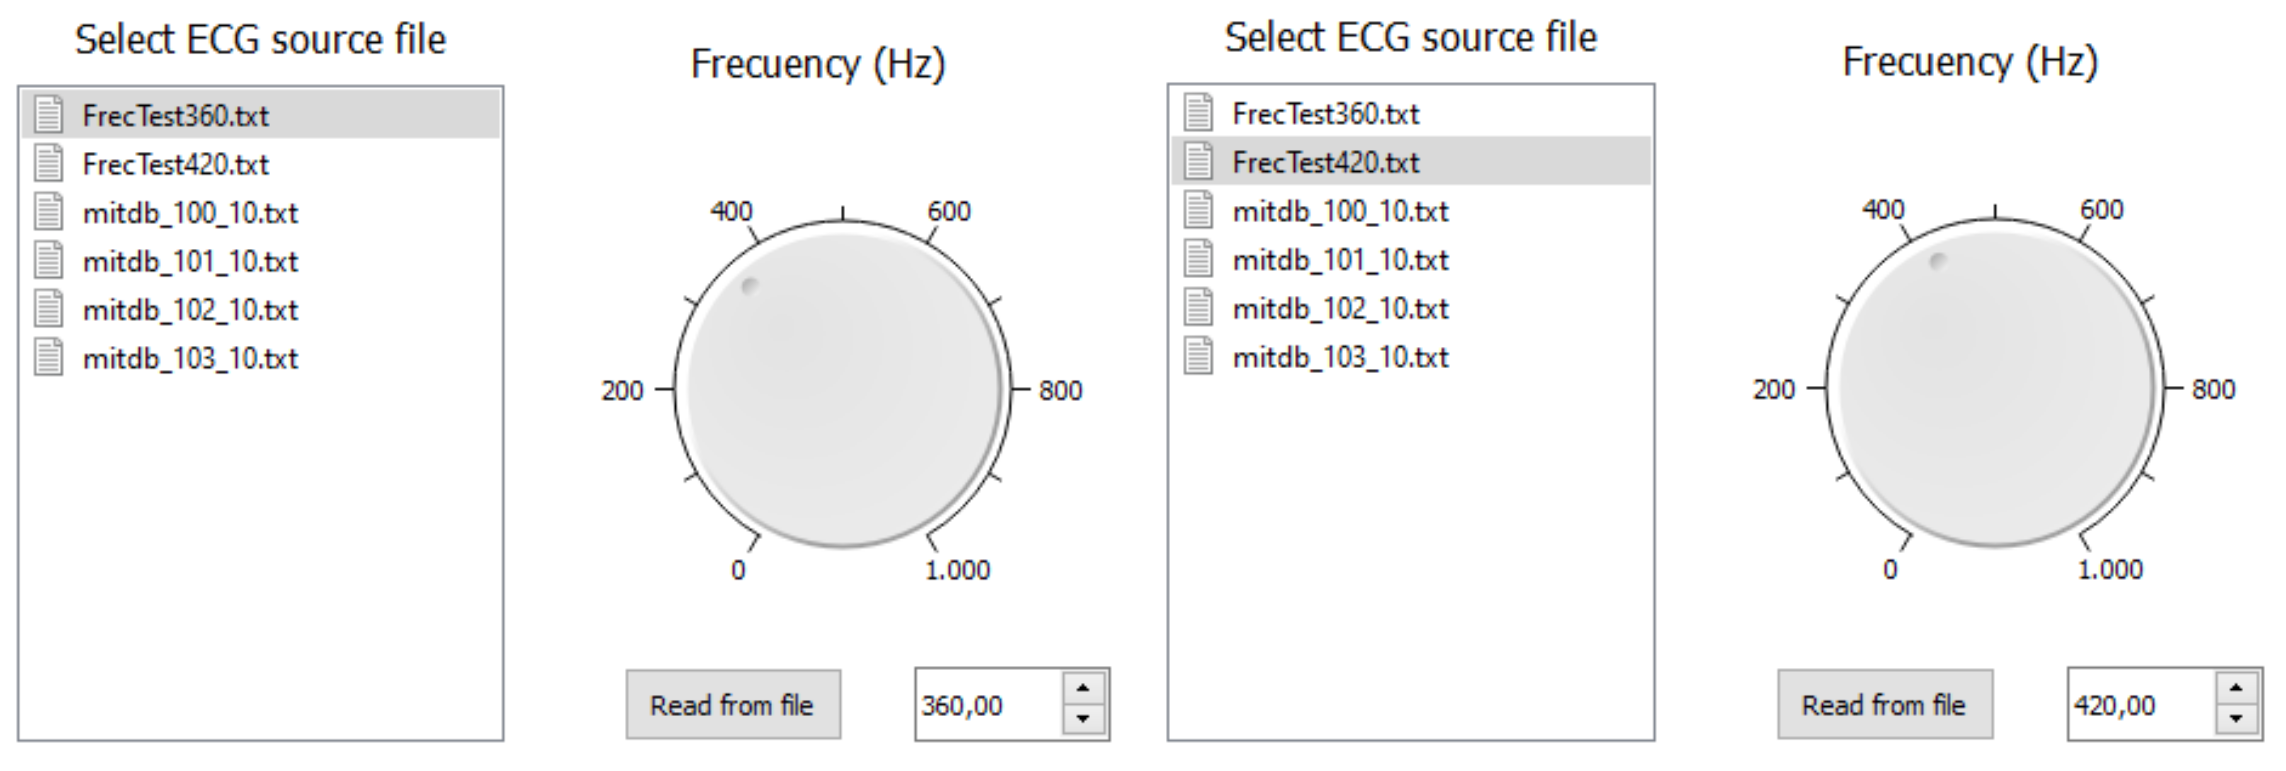
\includegraphics[width = \linewidth]{figuras/FileSelectorTest.png}
                \caption{Lectura de diferentes ficheros desde el selector.}
                \label{fig:fileSelectorTest}
        \end{figure}

        TODO: Escribir un test del buffer

        Para testear la interfaz, o mejor dicho, el puntero a una función simplemente se ha ejecutado el código en modo debug y comprobado que en el momento apropiado este ejecutaba la función correctamente mediante un punto de ruptura. 

        El test correspondiente al envío de los resultados de vuelta al panel resulta ser más sencillo de lo que pueda parecer a priori. Pues el envío correcto de los datos no implica que los datos sean correctos, por lo que no es necesario tener de momento un algoritmo capaz de detectar eficazmente la tasa cardiaca. Comprobando mediante puntos de ruptura que el dato enviado y recibido son el mismo y chequeando visualmente que el dato mostrado también es coherente puede darse por concluida esta prueba.

        
    \subsection{Conclusiones}
    
        Con la finalización de esta iteración queda definida la funcionalidad general, sin embargo para gozar de un primer prototipo cerrado es necesario llevar a cabo algunos cambios en el futuro cercano.
        
        Actualmente la interfaz para el algoritmo se ejecuta dentro de la rutina de recepción de los mensajes. Aunque es capaz de llevar a cabo todas la funciones que se le requieren sería más óptimo separar el procesado de la señal en una tarea aparte gestionada por el sistema operativo. Con esto se conseguiría además aislarla para simplificar la medida del rendimiento, permitiendo además emplear los propios mecanismos de FreeRTOS (TODO: Referencia a estos mecanismos) para realizar las medidas de rendimiento necesarias.
        
        Esta modificación se incluye como requisito en la tabla final (TODO: Referencia a la tabla final de requisitos) con el código: 2.5, aislamiento del procesado de señal.